\documentclass[preprint]{aastex}
\usepackage{amsmath, amsfonts, amssymb}
\usepackage[T1]{fontenc} % recommended magic command
\usepackage{microtype} % subtle improvements in PDF typography
\usepackage[colorlinks,urlcolor=blue,citecolor=blue,linkcolor=blue]{hyperref}

\slugcomment{Draft: \today}
\shorttitle{Rapid Primary Beam Characterization}
\shortauthors{Burns et al.}

\begin{document}
\title{Rapid Characterization of the Primary Beam Properties of
  Pointable Interferometric Array Elements}
\author{Keaton J. Burns, Peter K.~G. Williams, Geoffrey C. Bower}
\affil{Department of Astronomy, B-20 Hearst Field Annex~\#~3411,
  University of California, Berkeley, CA 94720-3411, USA}
\email{kburns@berkeley.edu}

\begin{abstract}
  High-fidelity wide-field interferometric imaging requires a precise
  understanding of the response patterns of the interferometric array
  elements. We present a technique for characterizing these patterns
  using a small mosaic of short observations around a bright,
  unresolved source. We describe the deployment of this technique at
  the Allen Telescope Array (ATA) and analyze measurements collected
  over a span of 17~months of routine observations. Our particular
  emphases are the individual beam shapes of the antennas, as modeled
  by two-dimensional Gaussians, and the ``squints,'' the separation
  between the effective pointing centers of the orthogonal linear
  polarizations received simultaneously by the ATA feeds. While the
  mean vertical polarization beam is round, we measure a small
  elevation elongation in the mean horizontal polarization beam, which
  we attribute to \textbf{clever explanation}. Although the squints
  display complex frequency-dependent behavior, there is generally a
  trend towards smaller squints at higher observing frequencies,
  indicating \textbf{other explanation}. Several revisions to the feed
  design reduced the typical squint magnitude and variability.
\end{abstract}

\keywords{Astronomical Instrumentation -- Astronomical Techniques}

%%%%%
\section{Introduction}\label{s.intro}

A common theme in the design of new and upgraded radio interferometers
is an emphasis on high survey throughput. Some undertakings, such as
the Apertif project at the Westerbork Synthesis Radio Telescope
\citep{theapertif} and the Australian Square Kilometer Array (SKA)
Pathfinder \citep[ASKAP;][]{theaskap}, achieve this by using
multi-element receivers on relatively few dishes. Others, such as the
Allen Telescope Array \citep[ATA;][]{Welch2009} and MeerKAT, the South
African SKA pathfinder \citep{themeerkat}, use ``large number of small
dishes'' (LNSD) array architectures to simultaneously attain good
sensitivity and large fields of view. Long-wavelength arrays, such as
the Precision Array for Probing the Epoch of Reionization
\citep[PAPER;][]{thepaper}, the Long Wavelength Array
\citep[LWA;][]{thelwa}, the Low-Frequency Array
\citep[LOFAR;][]{thelofar}, and the Murchison Wide-field Array
\citep[MWA;][]{themwa} take the LNSD paradigm to an extreme and have
designs calling for hundreds or thousands of dipoles that can be used
to image substantial fractions of the visible sky instantaneously.

These arrays are intended to produce accurate wide-field images of the
sky using either the mosaicking of many pointings or elements with
broad response patterns. In either case, a good understanding of the
receiving elements' response patterns is vital to the imaging process:
it has been shown that when imaging extended structures, small
($\sim$$10^{-2}$) inaccuracies in the response pattern model can have
enormous ($\sim$$10^2$) effects on image fidelity \citep{chu93,wc08},
and accurate response pattern modeling is also needed for correct
imaging of unresolved sources sitting between mosaic pointings.

Variation among array elements complicates matters. The most demanding
interferometric imaging applications already require substantial
calibration of per-element direction-dependent effects
\citep{bcgu08,ns10}. With the large numbers of elements in new
interferometers, more extreme outliers in the statistical variation
inherent in the manufacturing process will be encountered, and there
will be significant pressure to minimize per-element manufacturing
costs. In SKA-scale efforts \citep{theska}, with thousands of array
elements, budgetary realities will dictate that manufacturing
tolerances be as loose as they possibly can be without compromising
core scientific requirements. As such, it is vital to be able to
accurately characterize the response patterns of interferometric
elements and the effect that variations among these have upon the
overall scientific performance of an array.

In this work, we present a technique for measuring the response
pattern characteristics of the elements in an interferometer and
describe our implementation of it at the ATA. Our technique requires
pointable elements, and as such we couch our discussion in terms of
the primary beam (PB) shape of each element. A small mosaic of
pointings around a bright, unresolved calibrator is observed, with the
mosaic spacings approximately equal to the expected PB half-width at
half maximum (HWHM) of the array elements. Self-calibration
\citep{pr84} is used to derive relative per-element gains for the
offset pointings. If the calibrator dominates the observed flux, these
gains sample the PB response in particular off-axis directions, and
parametric models can be fit to these measurements to assess
properties such as PB HWHM and pointing offsets. An advantage of this
approach is that in a dual-polarization receiver system, the PB
properties of each polarization can be determined separately.

This paper continues a series of investigations of PB characterization
performed using the Allen Telescope Array. Analytical models of the
ATA PB based on the optical design are presented in \citet{wd04}. In
\citet{Hull2010}, independent images of mosaic pointings were used to
measure the aggregate PB of the entire array, with good agreement with
the theoretical predications. \citet{Harp2011} used holography to
perform extremely detailed measurements of the beam patterns of
specific array elements and analyze their dependence on factors such
as solar illumination, observing frequency, and the position of the
ATA's focusable feeds. The information provided by the technique
presented herein is much less detailed than what can be achieved with
the techniques of \citet{Harp2011}, but the necessary observations can
be performed in minutes rather than days, and thus our technique can
feasibly be used to monitor array performance. Unlike the method of
\citet{Hull2010}, our technique requires special observations, but
because it does not operate in the image domain, we can investigate PB
characteristics on an element-by-element basis rather than in the
aggregate.

We begin by describing the observations used to perform the PB
characterization (\S\ref{s.observations}). We then describe the
analysis technique used to extract PB information
(\S\ref{s.reduction}). Next, we present results describing the PB
sizes and polarization-based pointing offsets in the ATA
(\S\ref{s.results}). \ldots Finally, we present our conclusions
(\S\ref{s.conclusions}).

%ATA telescope calibration is accomplished through observing known
%radio point sources to determine the system temperature, pointing
%centers, and beam shape for each antenna.  One parameter of interest
%from these observations is telescope squint, which we define as the
%offset of the Y polarization pointing center from the X polarization
%pointing center, in azimuth and altitude.  Knowledge of each
%telescope's squint is useful for assessing the reliability of data
%from each polarization based on each telescope's pointing model
%(e.g., for large-squint telescopes, pointing models based on X
%polarization pointing centers yield suboptimal Y polarization
%data). Studying telescope squint also provides insights into the
%strengths and limitations of the offset-Gregorian dish and
%log-periodic feed designs used at the ATA, and may be useful for
%directing future telescope development.  Our aims in this project
%included isolating the cause of the squint to the feed or dish,
%studying the effects of feed upgrades on the squint, and assessing the
%stability of a telescope's squint with changes in frequency and time.

%%%%%
\section{Observations}\label{s.observations}

Measurements of PB shape and squint were obtained by weekly
observations of bright, unresolved sources from 2009~Oct~17 to
2011~Apr~06. The core observing pattern in each session consisted of
an observation pointed directly at the source followed by a small
mosaic of pointings offset from the source by an angle comparable to
half of the nominal PB full-width at half maximum (FWHM). Each
pointing lasted for 60--90 seconds, with a typical pattern taking
about 20 minutes to observe (including overheads). In the significant
majority of cases, the small mosaic consisted of six additional
pointings arranged in a equilateral hexagon around the central
source. Two points of the hexagon were on a line of constant
declination matching that of the source and the distance between
pointings was exactly half of the nominal PB FWHM. Other pointing
patterns, such as crosses or nested hexagons, and other offset sizes,
such as one quarter of the FWHM, were occasionally used.  The sources
3C\,48, 3C\,138, 3C\,147, and 3C\,286 were used as targets, with the
selection depending on visibility and higher-elevation sources being
preferred.

At the time of the observations, the ATA had two independently-tunable
correlators able to access any central frequency within the facility's
overall accessible band, 0.5--11~GHz. Each observing session included
several cycles of observing patterns with the correlators tuned to
several pairs of frequencies. Most observations were made with paired
central frequencies of 0.7 \& 1.43, 2.01 \& 3.14, or 5.00 \&
7.60~GHz. Each correlator had a bandwidth of 104~MHz divided into 1024
spectral channels.

Because the position of the focal point of the ATA optical path is
wavelength-dependent, each ATA feed is mounted on a piston that allows
repositioning of the feed for optimal match to one of the observing
frequencies. Feed performance degrades for frequencies above the
commanded ``focus frequency'' while it remains fairly good for those
below it \citep{Harp2011}. In these observations the focus was always
set to be optimal for the higher of each pair of observing
frequencies.

\section{Analysis}\label{s.reduction}

After each observing session the data were reduced with an automated
pipeline. The observation of the central pointing of each observing
pattern was automatically flagged for radiofrequency interference
(RFI) and gain- and bandpass-calibrated using the COMPASS system
developed for the ATA \citep{Keating2010}. The rest of the scans were
likewise automatically flagged and had the calibrations from the
central pointing applied. Some scans were discarded due to excessive
RFI or problems in digital hardware; if the central pointing was
discarded, the whole pointing pattern was as well.

Each ATA feed is sensitive to two orthogonal linear polarizations, $X$
(horizontal relative to ground) and $Y$ (vertical). Only parallel-hand
correlations were processed, so that the $X$ and $Y$ correlations were
effectively reduced independently. We refer to the signal originating
from a particular polarization on a particular antenna as coming from
a certain ``antpol''. In some antennas, only one antpol was
correlated.

After initial calibrations were applied, the MIRIAD \citep{Sault1995}
task \textsf{selfcal} was used on each side pointing to derive complex
correction gains for each antpol. An additional program was written to
determine uncertainties in the solved-for gains, which are not
reported by \textsf{selfcal}. Because the received flux in all fields
is dominated by the central calibrator source, these gains can be
interpreted as the inverse of the complex PB response associated with
each antpol in the direction of the calibrator, where the response
towards pointing center is unity. These gains may vary between antpols
on the same antenna due to differences in the spatial response of the
$X$ and $Y$ receptors or polarization leakage in the overall optical
path.

Two-dimensional (2D) Gaussian profiles in azimuth-elevation (az-el)
space were fit to the measurements of each antpol in each pointing
pattern. Because the pointing patterns on the sky were aligned to the
equatorial coordinate system, the az-el offsets probed varied as a
function of parallactic angle and did not trace out precisely uniform
figures. Each Gaussian fit had five free parameters: offsets in
azimuth and elevation from pointing center; characteristic widths in
azimuth and elevation; and an overall amplitude scaling. The fits
resulted in measurements of these parameters, their formal
uncertainties, and a reduced $\chi^2$ value for the overall
result. Other data products of the pipeline included the relative
complex gain values, post-hoc measurements of the system equivalent
flux density (SEFD) for each antpol, and images of the central
pointings.

\subsection{Squint Database}\label{ss.database}
For those antennas for which data from both polarizations were available, 
Gaussian fit parameters and squint vectors (calculated as defined in 
\S\ref{s.intro}) were imported into a relational database for analysis.

A query program use the Structured Query Language (SQL) to retrieve
and plot data with arbitrary filtering and transformation of the
underlying values. Derived data such as squint magnitudes and angles,
and their respective uncertainties, are computed during retrieval.

\subsection{Outlier Removal}\label{ss.outliers}
A mechanism was implemented to exclude bad data from downstream
analyses.  To remove bad observations, and particularly poor reduction
fits, observations with frequency-normalized squint or width
components above the 99$^\textrm{th}$ percentile, or uncertainties above the
98$^\textrm{th}$ percentile, were flagged as outliers.  Observations
above the 98$^\textrm{th}$ percentile of SEFD and the 90$^\textrm{th}$
percentile of the Gaussian fit $\chi^2$ value were also flagged.  The
$\chi^2$ cutoff is at a significantly lower percentile, as it is a
direct indicator of the convergence of the Gaussian fits, and there
were a significant number of outliers in this parameter, as shown in
Fig.~\ref{fig.dist_sumchisq}.

Over half of the observations at 700 MHz, the lowest observed frequency,
were flagged under these conditions, so the remaining observations
were also excluded.  After removal of
these data, 5040 observations remained.

\begin{figure}[htb]
\begin{center}
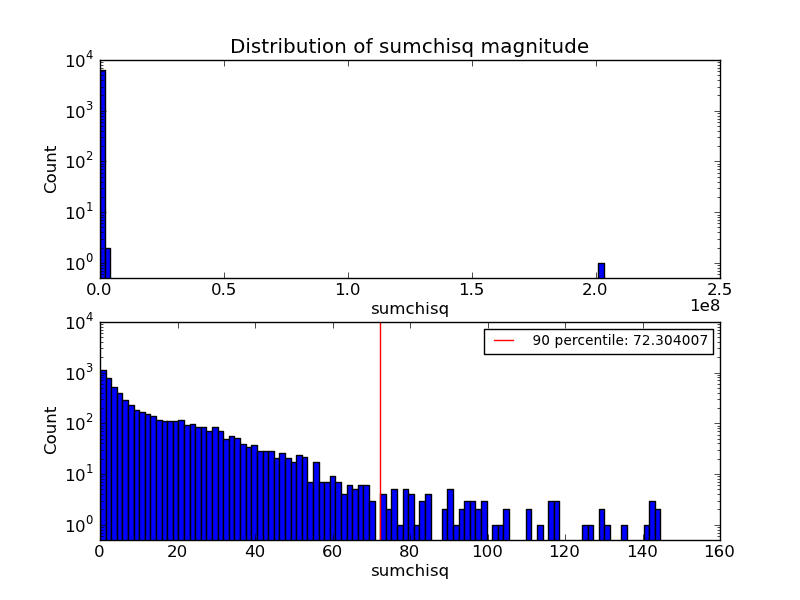
\includegraphics[width=0.7\textwidth]{images/dist_sumchisq}
\caption{Top: Distribution of $\chi^2$ values for 2D Gaussian primary
  beam fits across all observations.  Bottom: Zoom-in at outlier
  cutoff at the 90$\textrm{th}$ percentile. \label{fig.dist_sumchisq}}
\end{center}
\end{figure}


%%%%%
\section{Results}\label{s.results}

\subsection{Primary Beam Size}\label{ss.beamsize}
The PB shape distributions for the X and Y polarizations are depicted in 
Figures~\ref{fig.x_shape} and \ref{fig.y_shape}, respectively.  The beam size 
is given by the frequency normalized geometric mean of the azimuthal and 
elevation beam diameters.  The beam angle is arctangent of the elevation 
width divided by the azimuthal width. A $45\degr$ beam angle therefore 
corresponds to a circular beam and is indicated by a red line in the plots; a 
higher value corresponds to a beam elongated in elevation, and a
smaller value corresponds to a beam elongated in azimuth.

Table \ref{tab.beamshape} gives the means and standard
deviations of these values.  We find general agreement with the
approximate results of \citet{Harp2011}, namely $\textrm{FWHM} \approx
3.5\degr / f_\textrm{GHz}$, indicated by a red line in the plots.  We find 
that the Y polarization beams are generally round, with a mean beam angle 
lying 0.12 standard deviations from $45\degr$.  The X polarization beams 
show a systematic stretch in elevation, with a mean beam angle 1.11 
standard deviations above $45\degr$.

\begin{table}[htb]
\begin{center}
\begin{tabular}{cccc}
Parameter & Polarization & Mean & St. Dev \\
\hline
%X & El & 3.663 & 0.245 \\
%X & Az & 3.443 & 0.216 \\
%Y & El & 3.568 & 0.331 \\
%Y & Az & 3.568 & 0.303
Beam Size $[\degr / f_\textrm{GHz}]$ & X & 3.512(2) & 0.158 \\
  & Y & 3.517(2) & 0.176 \\ \hline
Beam Angle $[\degr]$ & X & 46.54(2) & 1.39 \\
  & Y & 45.19(2) & 1.59
\end{tabular}
\caption{Determined primary beam shape averages \label{tab.beamshape}}
\end{center}
\end{table}

\begin{figure}[htb]
\begin{center}
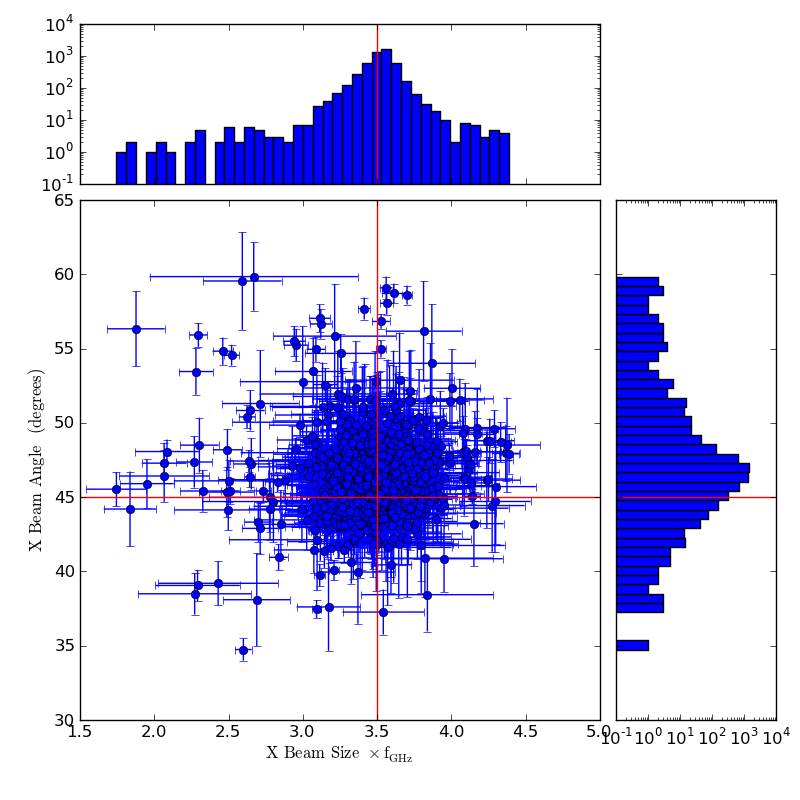
\includegraphics[width=0.8\textwidth]{images/x_magangle}
\caption{Scatterplot and logarithmic histograms of determined X
  polarization primary beam sizes and angles. \label{fig.x_shape}}
\end{center}
\end{figure}

\begin{figure}[htb]
\begin{center}
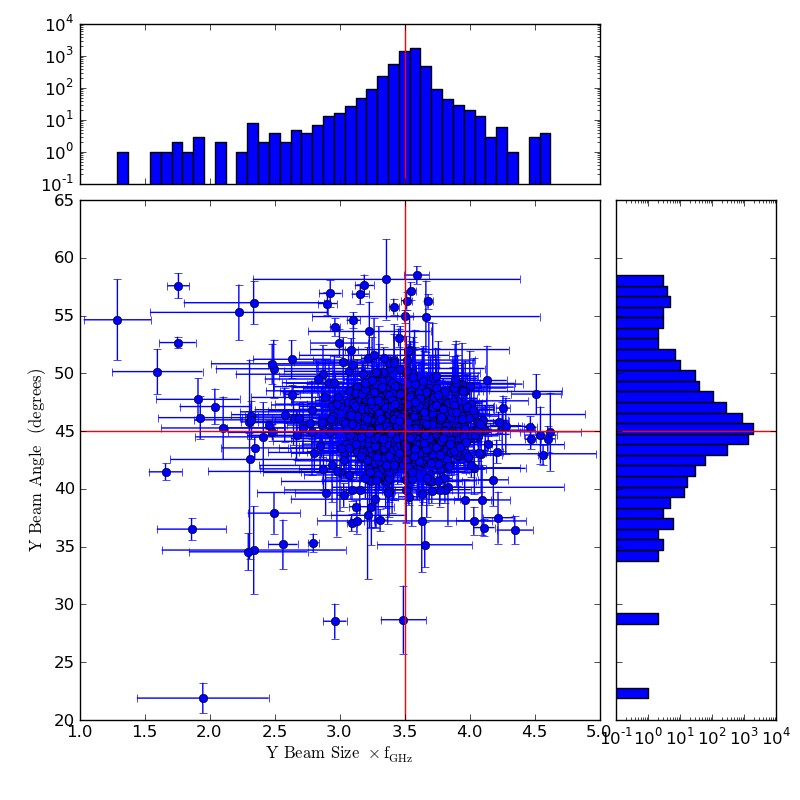
\includegraphics[width=0.8\textwidth]{images/y_magangle}
\caption{Scatterplot and logarithmic histograms of determined Y
  polarization primary beam sizes and angles. \label{fig.y_shape}}
\end{center}
\end{figure}

\subsection{Squint Stability}\label{ss.temporal}
The temporal stability of telescope squint is an important factor in 
determining the required cadence of pointing calibrations.  For each ant 
feed and frequency, we took the standard deviation of squint magnitude 
over time, and normalized to the mean squint magnitude across the same 
dataset.  This measurement represents the relative instability of squint 
magnitude for a given ant feed and frequency.  Histograms of these 
fractional standard deviations for each feed revision are displayed in Fig.~
\ref{fig.squint_time}.  The successive revisions appear to improve squint 
stability, with the average fractional standard deviations decreasing from 
0.44 to 0.35 from the first to third revisions.  However, the sample sizes for 
these measurements are relatively small: 135, 75, and 49 for the respective 
revisions.  

\begin{figure}[htb]
\begin{center}
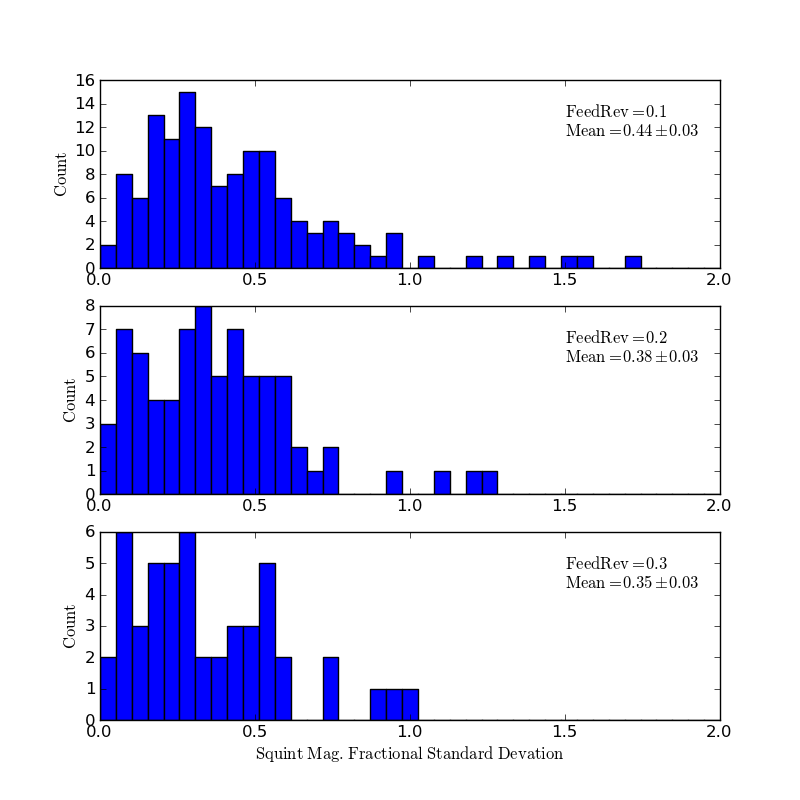
\includegraphics[width=0.8\textwidth]{images/squinttime_rev}
\caption{Normalized standard deviations of squint magnitude over time,
  for each antfeed and frequency, separated by feed
  revision. \label{fig.squint_time}}
\end{center}
\end{figure}

\subsection{Squint: Frequency Dependence}\label{ss.freq}
To study the effects of frequency on squint, for each antfeed, we
performed a linear least-squares fit on the log of squint magnitude
and the log of frequency for each observing run.  The slope of this
fit represents the best fitting power-law index $\alpha$, assuming
$|\vec{S}| \propto f^\alpha$.  Power law indices greater than 5 in absolute 
value were discarded as outliers (22 of the 1256 measurements).

Histograms of the remaining indices for each feed revision are displayed in 
Fig.~\ref{fig.powerlaws}.  We notice substantial spread in the power-law 
indices, with means between -0.5 and -1.0, and standard deviations near 
1.0 for each feed revision.  In particular, the difference in the means 
between revisions are several times smaller than the standard deviations 
within each revision. We are therefore unable to discern any improvement in 
squint scaling across feed revisions.

\begin{figure}[htb]
\begin{center}
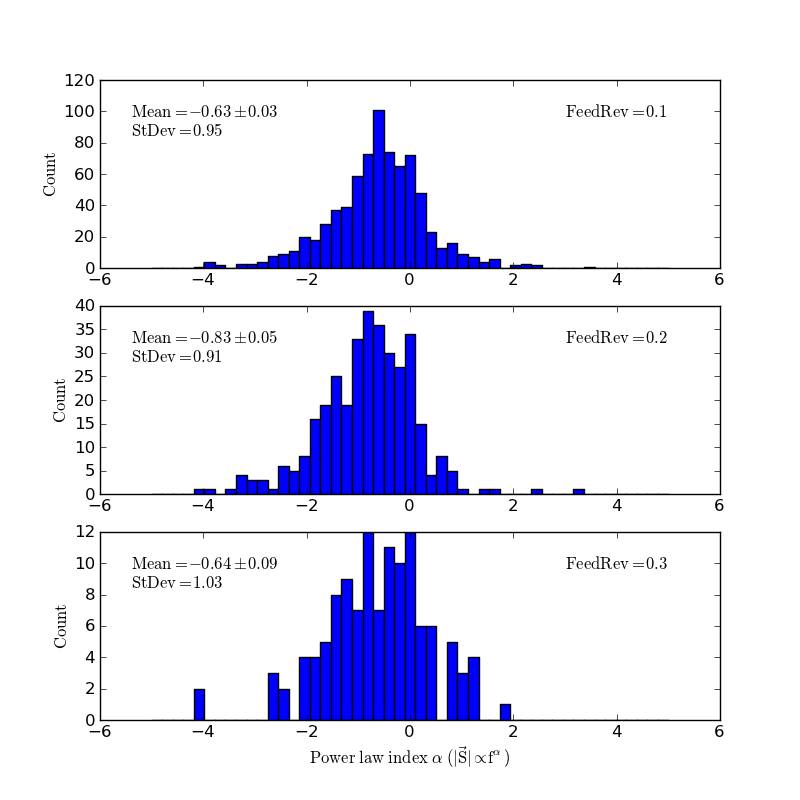
\includegraphics[width=0.8\textwidth]{images/powerlaw_rev}
\caption{Best-fit power law indexes of squint magnitude as a function
  of frequency, for each antfeed and observing day, separated by feed
  revision. \label{fig.powerlaws}}
\end{center}
\end{figure}

%%%%%
\section{Conclusions}\label{s.conclusions}
What did we learn?


%%%%%
\acknowledgments
Research with the ATA is supported by the Paul G. Allen Family
Foundation, the National Science Foundation, the US Naval Observatory,
and other public and private donors. This research has made use of
NASA's Astrophysics Data System.

Facilities: \facility{ATA}

\bibliographystyle{yahapj}
\bibliography{ATA.bib}

\end{document}
